\chapter{Big Data\label{ch:data}}

The LHC delivers $pp$ collisions at a high rate that is much higher than CMS can read out or store
offline. From all these collisions, CMS selects a small fraction of events
which are the most relevant for the physics processes of interest. This task is accomplished
through the trigger system, which is discussed in Section~\ref{sec:trigger} both in general and
in the context of this analysis. The events selected by the trigger system compose the datasets
used by all CMS analyses. The worldwide computing grid for storage and processing of both datasets
and simulation samples is discussed in Section~\ref{sec:storage}. Finally, the simulation samples
employed by this analysis are discussed in Section~\ref{sec:sim}.


\section{The Trigger System\label{sec:trigger}}

The gap in time between successive bunch crossings by the LHC is 25 ns, equivalent to
a frequency of 40 MHz. This large rate is reduced by selecting only the most interesting events
that pass a two-level trigger system. The first level, Level 1 (L1), is hardware-based and reduces the
total event rate from 40 MHz to 100 kHz~\cite{Bayatyan:706847}, whereas the second level,
the High Level Trigger (HLT), is software-based and reduces the total event rate from 100 kHz to
100 Hz~\cite{Virdee:1043242}. From here, the events are processed further and stored
for the physics analyses.

The L1 trigger attempts to identify basic physics objects based on coarse energy deposits in
ECAL or HCAL or
based on collections of hits in the muon chambers.
Quantities derived from the sum of energy deposited, such as the missing transverse energy $\met$,
provide other quantities on which to characterize events.
The Level 1 global trigger (GT) combines these object candidates and derived quantities in order
to select events to pass the the HLT with a processing time of $3~\mu$s.
Up to 128 separate trigger paths can be supported, 126 to 127 of which were used during 2012
data taking. %https://twiki.cern.ch/twiki/bin/view/CMS/GlobalTriggerMenu_L1Menu_Collisions2012_v1

The HLT is able to access more information than the L1 trigger, and in doing so it can provide
a better description of the event. At the HLT level, tracker information is used in conjunction with
the full granularity of ECAL and HCAL. Information at this level is based on the presence of one or
more candidate objects satisfying requirements based on their transverse momentum or energy and relative
or absolute positions in the detector. With this added complexity and fewer events to process,
the average processing time is 40 ms per processor.

\subsection{The Trigger for $\ggbb$}

The search for the $\ggbb$ final state can be viewed as an extension of the
SM $\Hgg$ search~\cite{HggCMSpaper}. The excellent diphoton mass
resolution is the primary driver in the sensitivity, since it allows for low background contamination
in the signal region, as will be shown in Chapter~\ref{ch:signalextraction}.
Therefore, the trigger strategy centers on the ability to find two high-quality photon candidates.

During 2012 data taking, the LHC luminosity increased over time, and the triggers at both L1 and HLT
had their thresholds increased in order to keep the event rates within limits.
The requirement at L1 is for two $e/\gamma$ candidates with $E_{\rm T}$ requirements of 13 (7) GeV
for the leading (subleading) candidate or for one $e/\gamma$ candidate with an $E_{\rm T}$ requirement
of 22 GeV. Note that at this level, there is no distinction between electron and photon candidates as
the tracker information is not yet used.

Events are selected in the HLT through diphoton triggers with asymmetric $E_{\rm T}$ thresholds
and complementary photon selections. One trigger selection requires a loose calorimetric
identification based on the shape of the electromagnetic shower and loose isolation requirements
on the photon candidates, while the other requires that the photon electromagnetic shower
is primarily concentrated in a three-by-three crystal super-cluster.
The trigger thresholds on the photon $E_{\rm T}$ are 26 (18) GeV and 36 (22) GeV on the leading
(subleading) photon, depending on the acquisition period of LHC data taking in 2012.
The path with the 26 (18) GeV thresholds is initiated by the L1 path with 13 (7) GeV thresholds, while
the path with 36 (22) GeV thresholds is initiated by the L1 path with a single 22 GeV threshold.

In addition to keeping the trigger rate within its limits, it is also necessary to set thresholds
low enough such that the selection of signal events, or trigger efficiency,
remains as high as possible. The trigger efficiency
is studied on Monte Carlo (MC) signal samples as well as on $Z\rightarrow e^+ e^-$ data.
According to the MC study, the efficiency is above 99.5\% for all conditions of 2012 data taking.

Figures~\ref{fig:ZeeTriggerPt} and \ref{fig:ZeeTriggerNvtx}
show how the trigger efficiency varies on data with respect to the
candidate photon $p_{\rm T}$ and the number of primary vertices in the event
using the tag and probe technique. To account for differences
in the shower shape between photons and electrons, the data sample was reweighted such that the shower
shape distributions match.
Within uncertainties, the trigger efficiency is higher than 99\% for the 2012 data.

\begin{figure}[htbp!]
 \begin{center}
    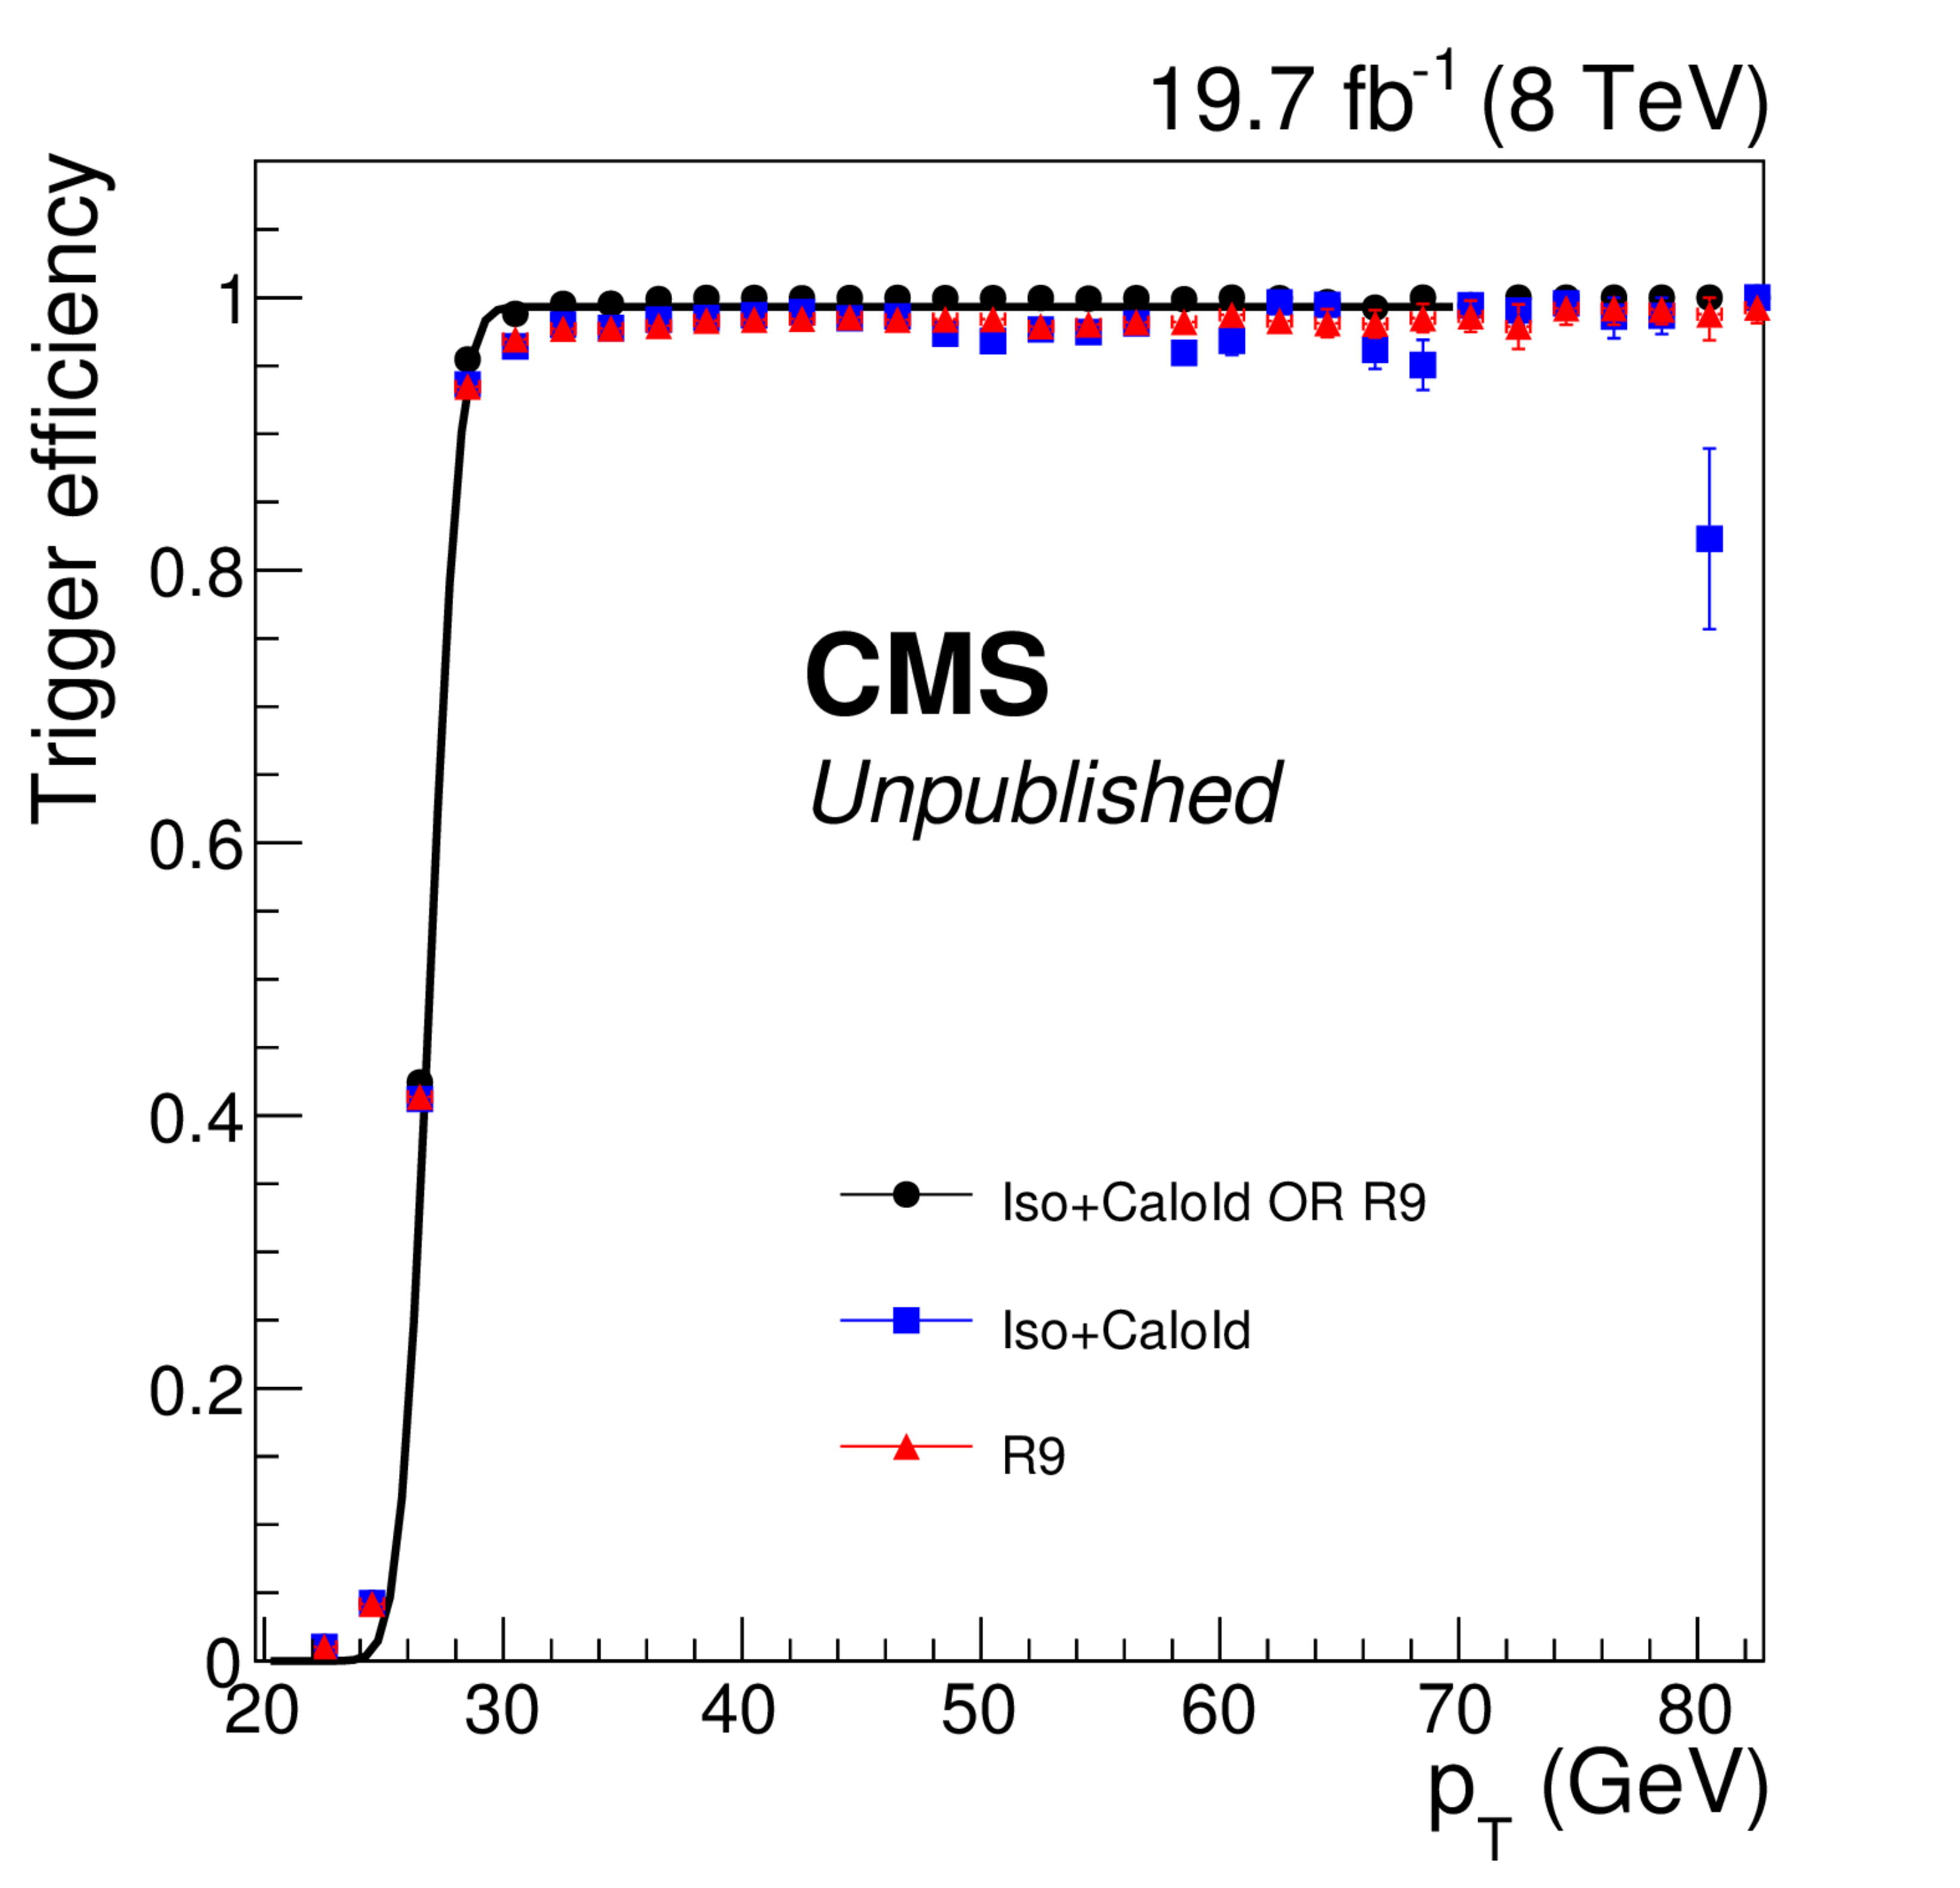
\includegraphics[width=0.60\textwidth]{figures/data/turnon_pt.pdf}
      \end{center}
\caption{Efficiency of the trigger selection as a function of the photon candidate transverse
momentum measured in $Z\rightarrow e^+ e^-$ events~\cite{HggCMSpaper}.}
\label{fig:ZeeTriggerPt}
\end{figure}

\begin{figure}[htbp!]
 \begin{center}
    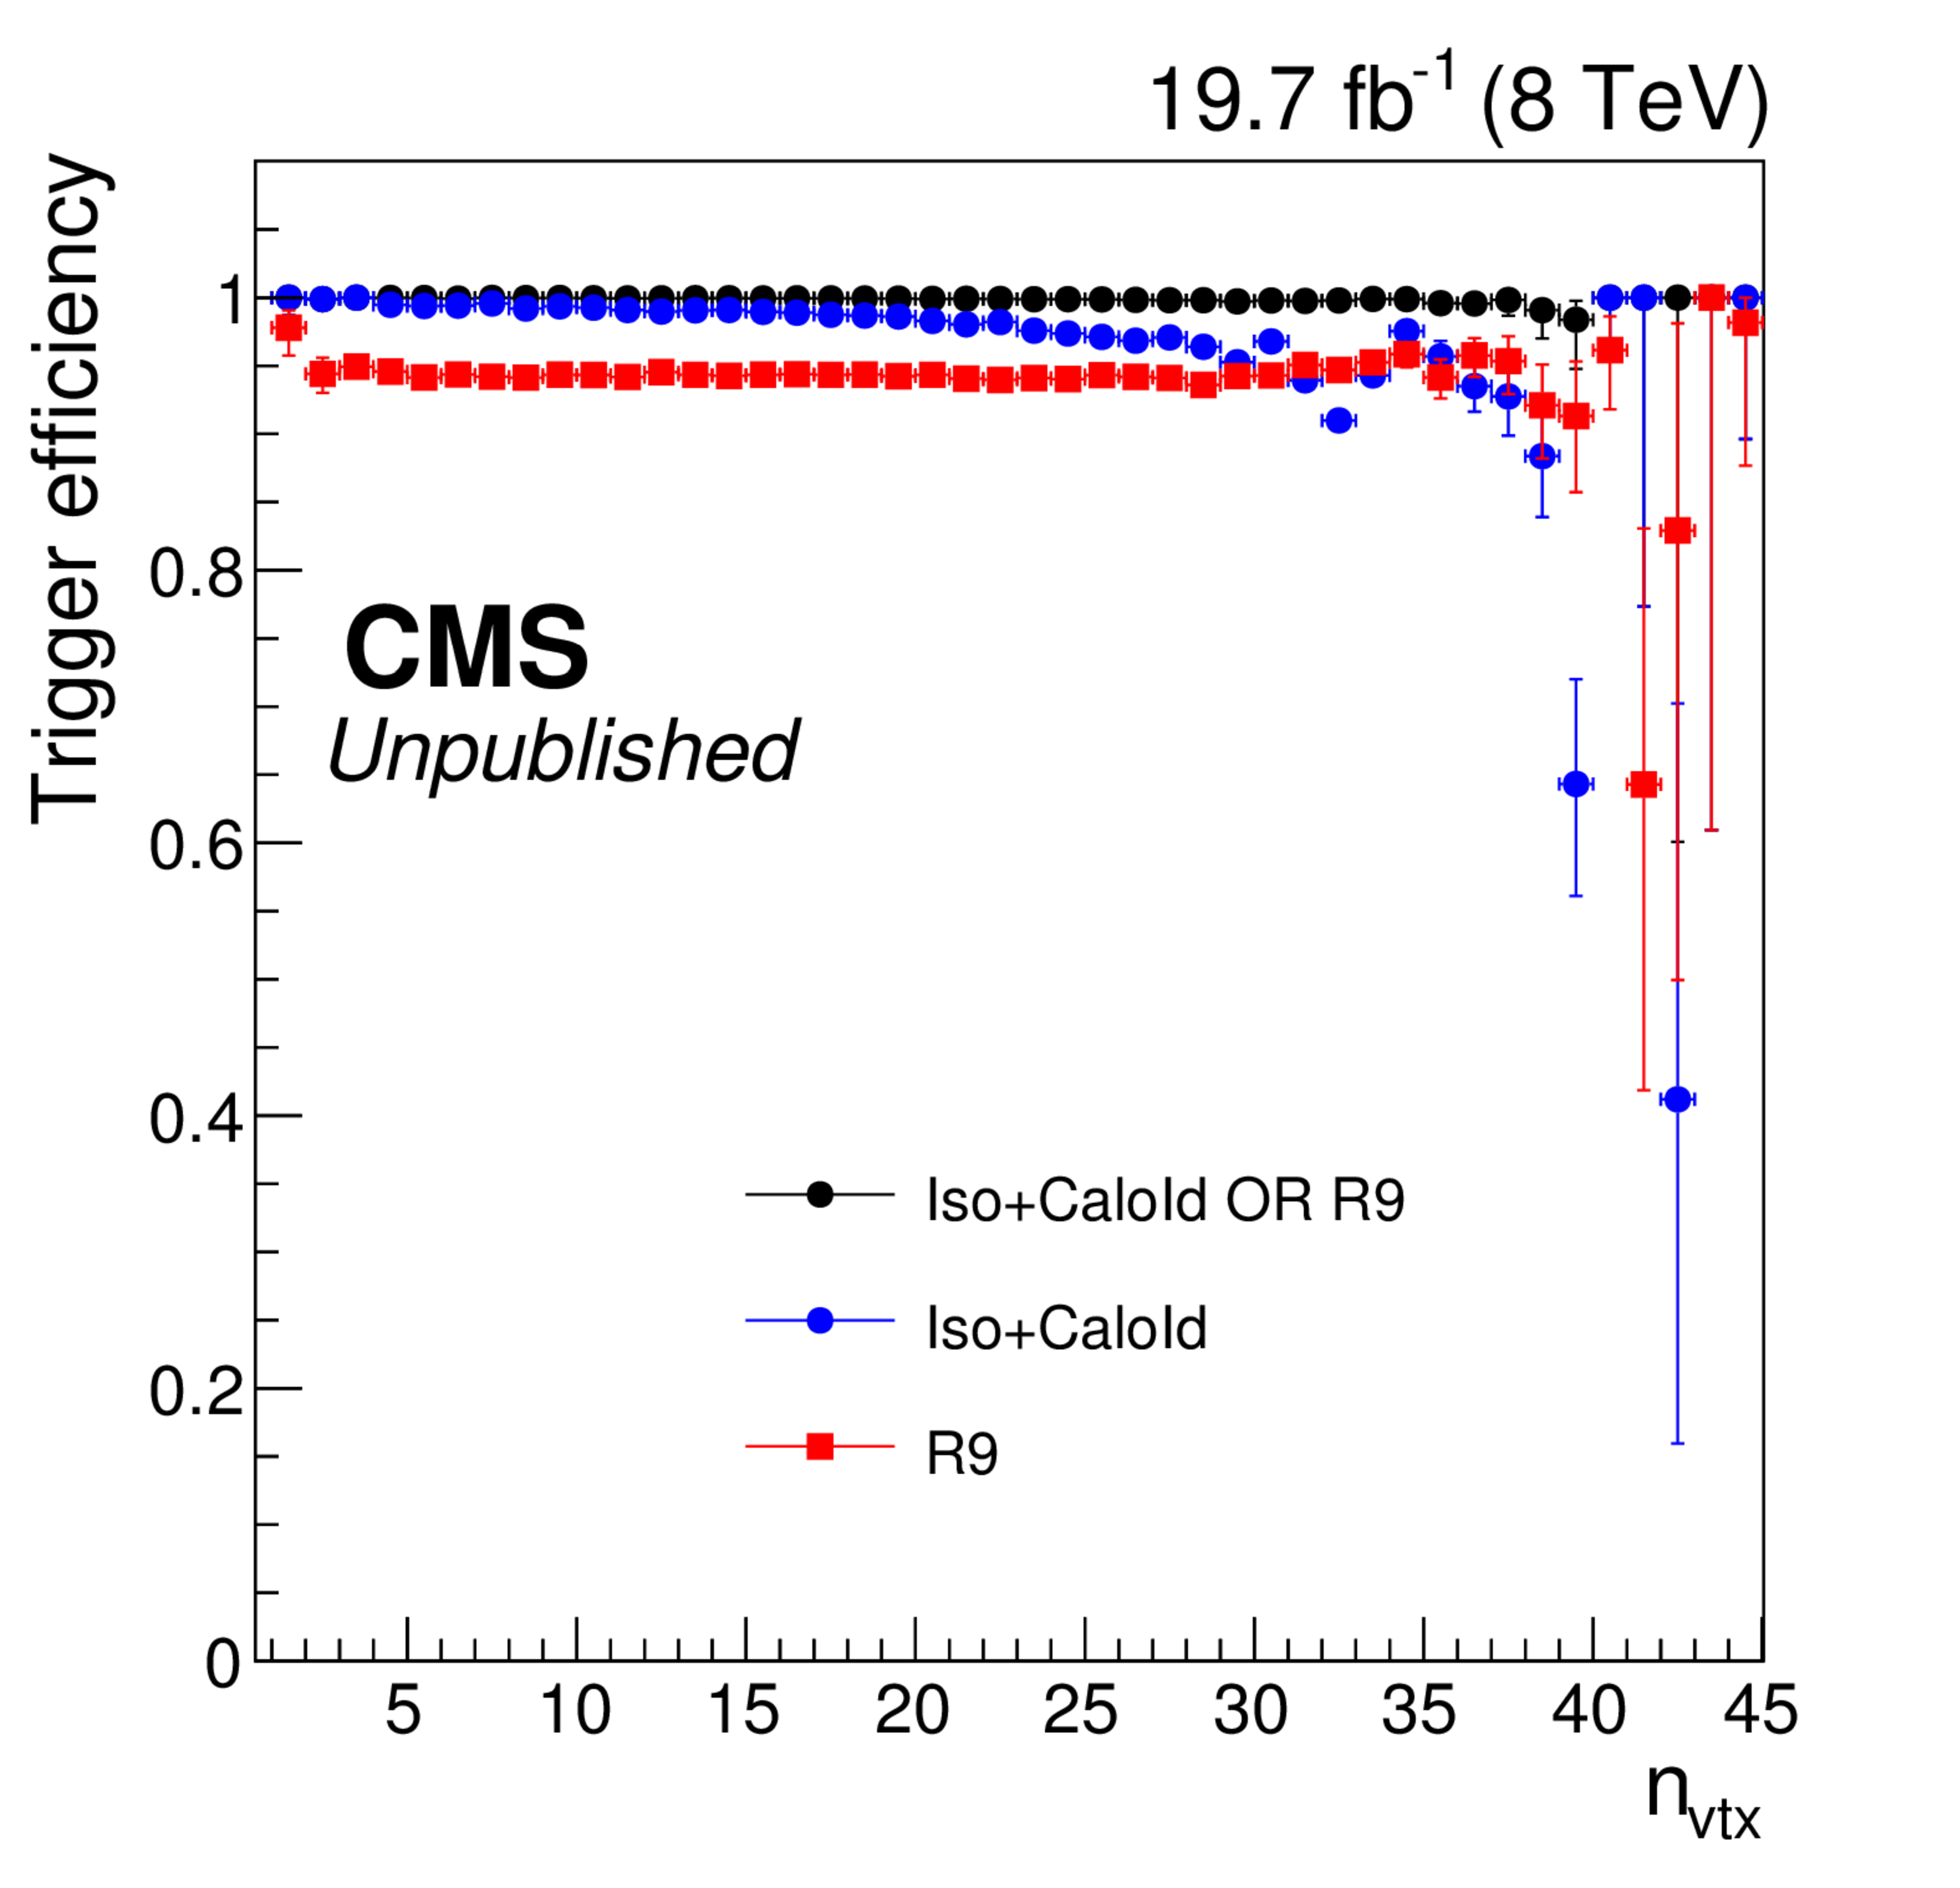
\includegraphics[width=0.60\textwidth]{figures/data/turnon_nvtx.pdf}
      \end{center}
\caption{Efficiency of the trigger selection as a function of the number of primary vertex in the event
measured in $Z\rightarrow e^+ e^-$ events~\cite{HggCMSpaper}.}
\label{fig:ZeeTriggerNvtx}
\end{figure}


\section{Data Storage Worldwide\label{sec:storage}}

All the data from the LHC and its experiments, including CMS, is processed, stored, and analyzed
in a distributed global collaboration of computing centers~\cite{Eck:840543}. The Worldwide
LHC Computing Grid (WLCG) is the world's largest computing grid, comprising over 170 centers
arranged in a structure of tiers. Part of this tier structure is shown in Figure~\ref{fig:cerncomputing}

\begin{figure}[htbp!]
 \begin{center}
    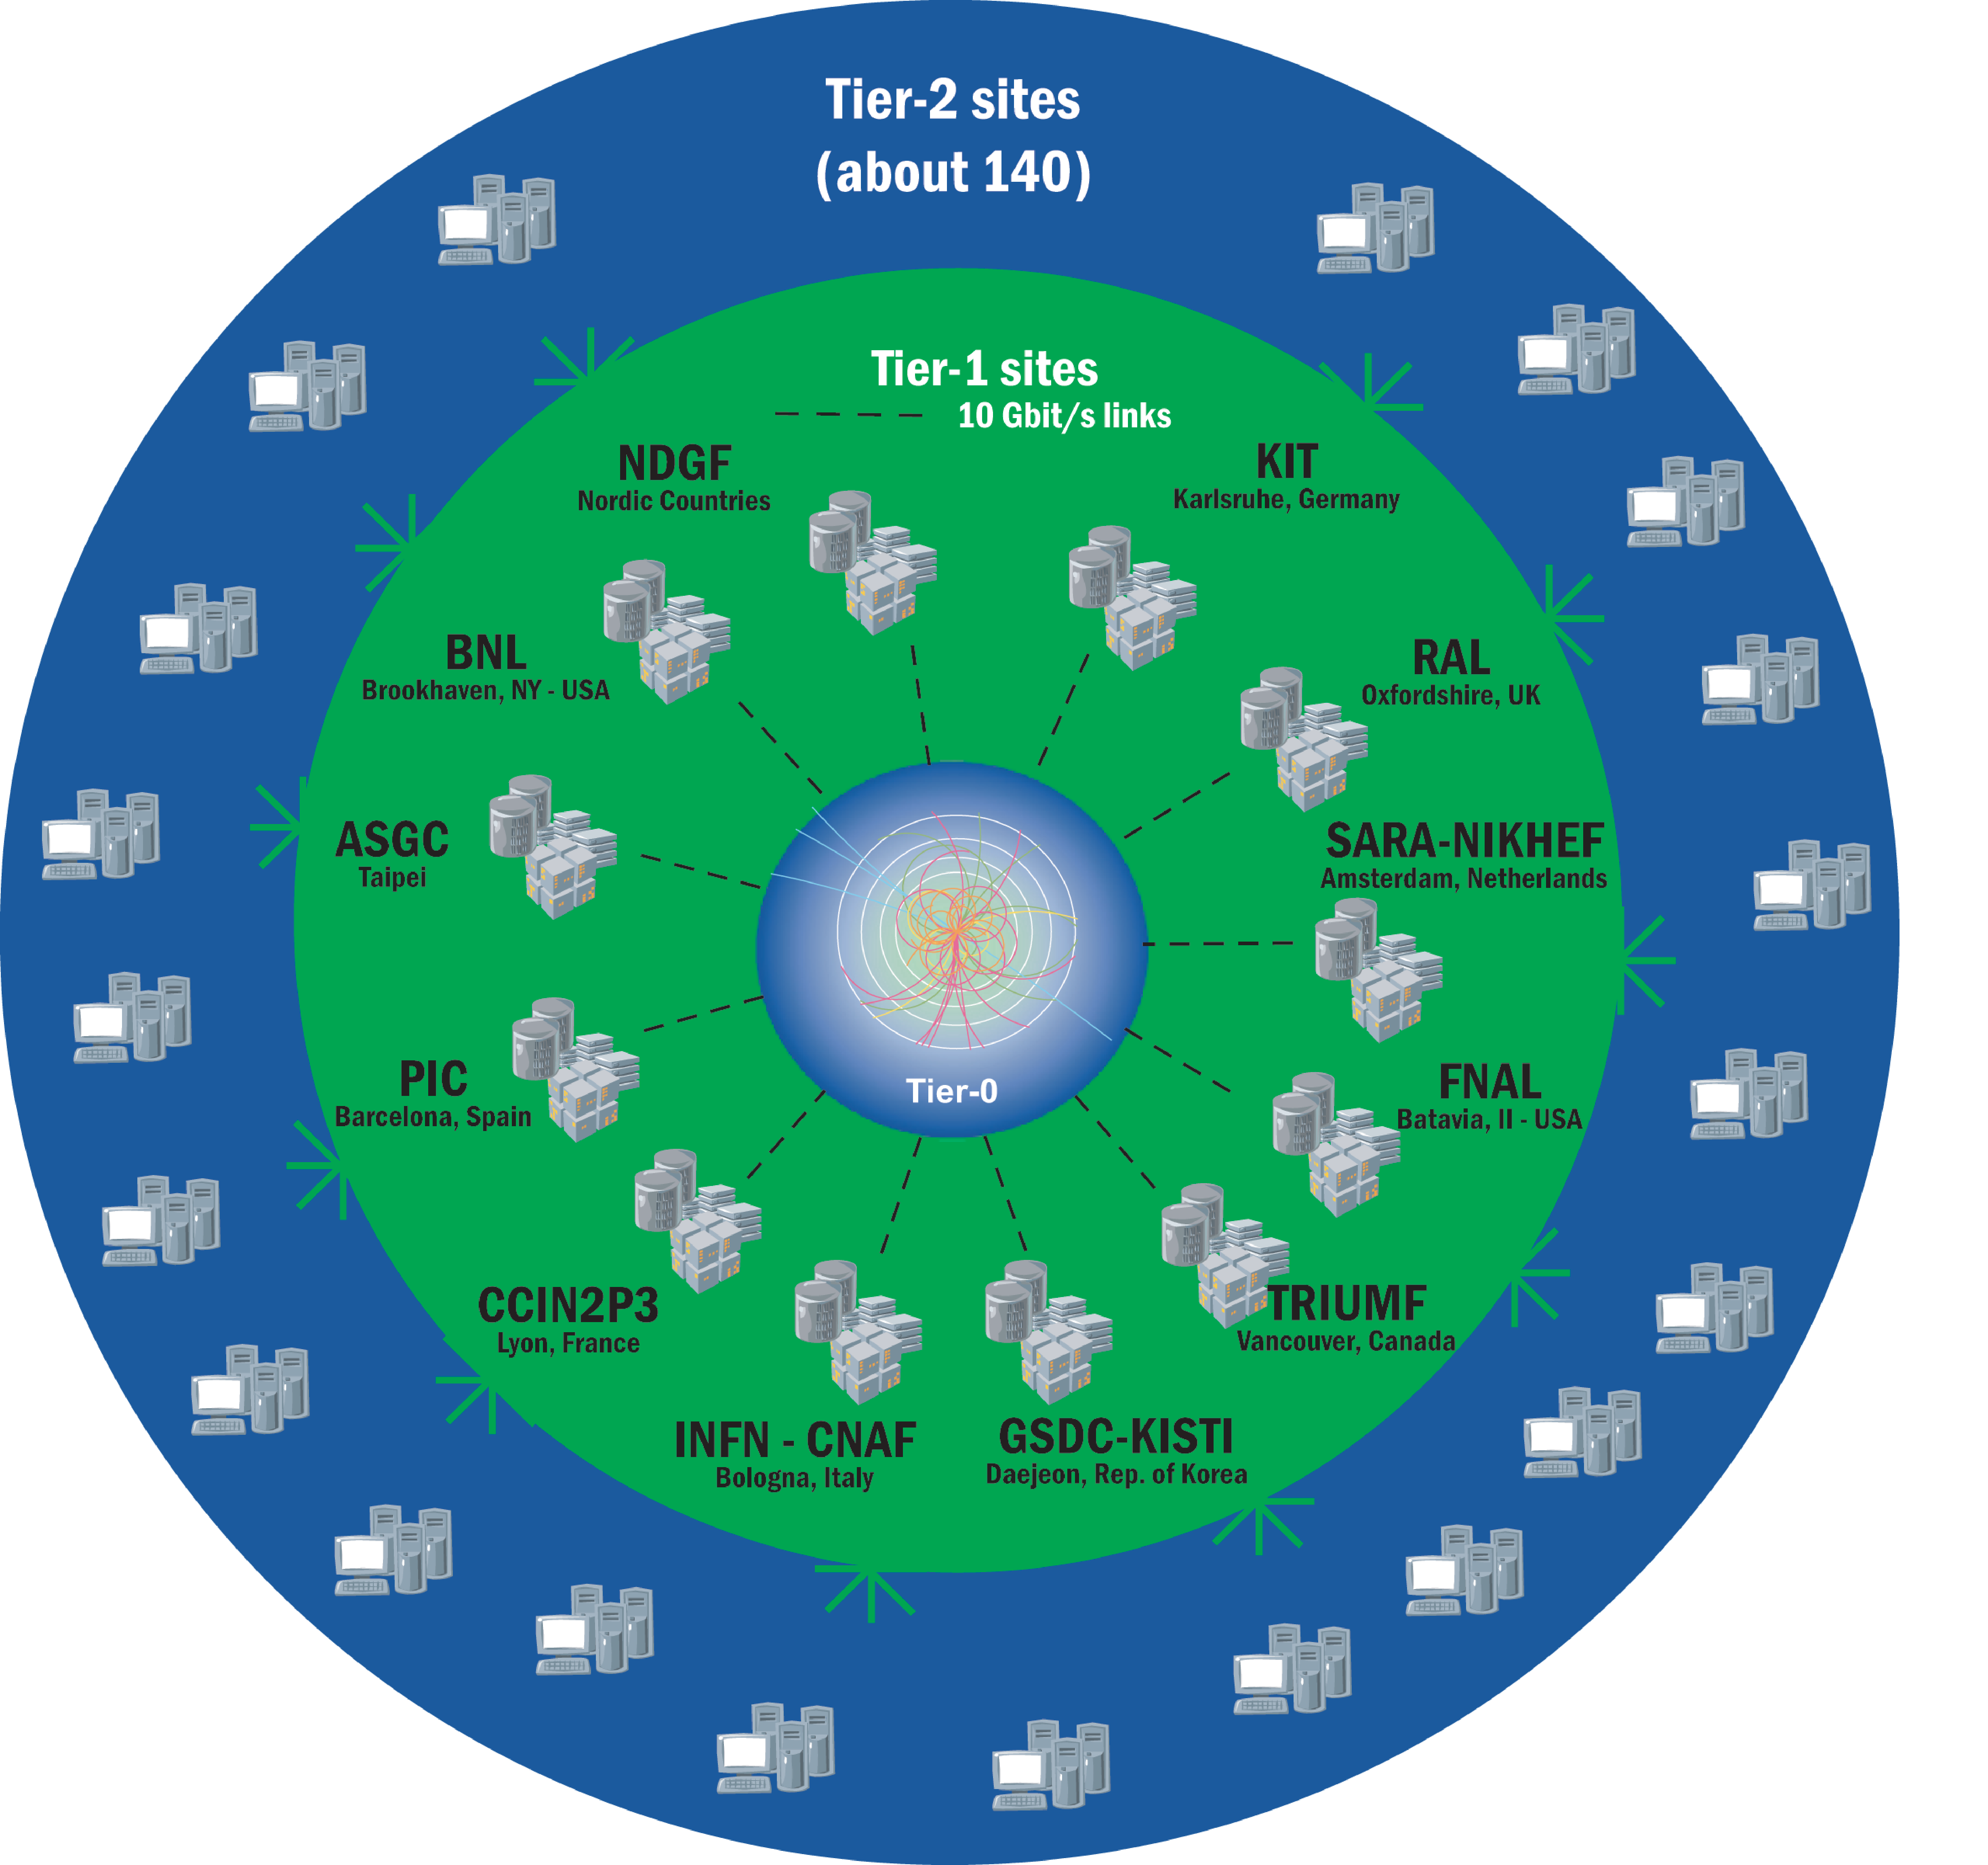
\includegraphics[width=0.80\textwidth]{figures/data/CCApr13-Tiers0-1-2_PNG-file.pdf}
      \end{center}
\caption{A schematic of the WLCG detailing the locations of the Tier-1 sites~\cite{cern:computing}.}
\label{fig:cerncomputing}
\end{figure}

Tier 0 is the CERN Data Center, through which all LHC data passes for initial processing and
reconstruction. For CMS, this comprises the events that pass the HLT.
The raw and processed data from Tier 0 is pushed to one of the 13 Tier 1 sites, where
later reprocessing and storage can be done. From here, the Tier 1 sites push the reconstructed
datasets to Tier 2 sites for storage and processing by analysts. This system handles the approximately
30 Petabytes of data generated per year by the LHC experiments in addition to the large number of
MC samples generated and stored.

\section{Simulation Samples\label{sec:sim}}

%include more theory details on radion, graviton, mssm used in the sample generation

In a general search, MC simulation samples are employed to study the signal process of interest.
They also allow for the study of background processes in more detail
than would be offered by data alone.
This analysis searches for a double Higgs final
state by optimizing strategies separately between the resonant and
SM nonresonant production mechanisms.
The signal MC samples are discussed in Section~\ref{subsec:sig_samples}.
In addition, good agreement between data
and background MC confirms that the major backgrounds are understood and that
the data is behaving as expected. The background MC samples are discussed in
Section~\ref{subsec:bkg_samples}.

Event generation begins with sampling the probability distribution
estimated from the matrix element of the hard subprocess of interest
(for example, $gg\rightarrow HH\rightarrow \ggbb$). The matrix element
might have many contributions at tree level and, at higher orders, integrals involving loops, rendering
an exact calculation computationally infeasible.
From the hard subprocess, additional effects are added so that the simulation corresponds with
the final state observed in the detector. These effects include the initial state radiation (ISR)
and final state radiation (FSR) of a gluon or photon to the hard subprocess, multi-parton
interactions (MPI) from other parton interactions in the proton-proton collision with their
associated ISR and FSR, and beam remnants from the outgoing protons. Due to color confinement,
the partons cannot exist individually, and hadrons are formed from the bare partons in
a process called hadronization. Unstable hadrons decay further until more stable hadrons are
produced. The clustering of the stable hadrons observed in the detector give an inference of the
momentum of the parton produced in the hard subprocess.
More detail on the generation of simulation samples is provided in \cite{Dobbs:2004qw,Bartalini:2011jp}.

\subsection{Signal Simulation\label{subsec:sig_samples}}

The resonant search is focused on a new resonance from a massive particle $X$ with mass $m_X$ between
260 GeV and 1.1 TeV. The lower bound is set by twice the Higgs mass since the search looks for decays
$X\rightarrow HH$. The upper bound is set by the ability to reconstruct the $\ggbb$ final state: for
very high resonance hypotheses, the decay products are highly boosted, causing the photons of the
$\Hgg$ decay to fail identification and causing the jets of the $\Hbb$ decay to overlap.
These reconstruction methods are discussed in Chapter~\ref{ch:objects}. For the nonresonant
search, the final state is not sufficiently boosted to cause problems. The lack of boost in that
search is due to the distribution of the four-body mass being lower than that for
a high-mass resonance, where the spectrum is narrowly peaked about the resonance mass.

In the resonant search, the benchmark model is that of the Radion, which is simulated with
MadGraph5~\cite{Madgraph_Alwall:2011uj} and hadronized with Pythia6~\cite{Pythia6-0}. The events are
generated from the gluon-fusion production of an on-shell Radion where the decay width of the Radion
is 10 MeV, much less than the experimental resolution. There are roughly
20k events generated per mass point, with twice the number at three points.
This is summarized in Table~\ref{table:radion_mc} with the corresponding cross sections given in terms
of parameters described in Chapter~\ref{ch:intro}.

\begin{table}[htbp!]
  \centering
  \renewcommand{\arraystretch}{1.4}
  \caption{Radion simulation samples and their corresponding cross sections.}
  \begin{tabular}{|c|c|c|}
\hline
\multicolumn{3}{|c|}{ $\Lambda_R = 3$~TeV, $kl = 35$, no $R-H$ mixing}\\ \hline \hline
Mass $m_X$ (GeV) & Number of events & $\sigma \cdot BR(R\rightarrow HH \rightarrow \ggbb)$ (fb) \\
\hline
270 & 19996& 2.18 \\
300 & 39999& 1.94\\
350 & 18498& 1.19 \\
400 & 19697& 0.621 \\
450 & 19999& 0.402 \\
500 & 39997& 0.282 \\
550 & 19995& 0.206 \\
600 & 18197& 0.156 \\
650 & 20000& 0.121 \\
700 & 39995& 0.095 \\
800 & 19999& 0.0626 \\
900 & 19996& 0.0435 \\
1000& 19996& 0.0317\\
1100& 19400& - \\
\hline
\end{tabular}

  \label{table:radion_mc}
\end{table}

In order to verify the model-independence of the result, two additional resonant signals
are generated.
The spin-two graviton is considered as the angular distribution of the final state differs from a
spin-zero scenario. However, due to the expected sensitivity of the analysis, as shown in
Chapter~\ref{ch:results}, the analysis is not expected to be able to differentiate between
these two scenarios. %This will be explicitly checked in Chapter~\ref{ch:results}.
These samples were generated with a decay width of 1 GeV and 10 GeV,
which allows for the assessment of the
dependence of the decay width on the final result. The production mechanism is through
gluon-gluon fusion, generated with MadGraph5 and hadronized with Pythia6. The sample generation
is summarized in Table~\ref{table:graviton_mc} with corresponding cross sections given in terms of
parameters described in Chapter~\ref{ch:intro}. Here, the RS1 KK-graviton refers to a scenario
where $c_i = 1$ in Equation~\ref{eq:wed_lagrangian}, whereas the bulk KK-graviton refers to a scenario
in which the couplings between light quarks and the graviton are suppressed, causing the
production cross section of the bulk KK-graviton to be lowered by a factor of 0.02 from the
RS1 KK-graviton. The cross sections are given in Table~\ref{table:graviton_xsec}.

\begin{table}[htbp!]
  \centering
  \renewcommand{\arraystretch}{1.4}
  \caption{Graviton simulation samples.}
  \begin{tabular}{c | c}
Mass $m_X$ (GeV) & Width $\Gamma$ & Number of events \\ \hline
270 & 19996\\
300 & 39999\\
350 & 18498\\
400 & 19697\\
450 & 19999\\
500 & 39997\\
550 & 19995\\
600 & 18197\\
650 & 20000\\
700 & 39995\\
800 & 19999\\
900 & 19996\\
1000& 19996\\
1100& 19400\\
\end{tabular}

  \label{table:graviton_mc}
\end{table}

\begin{table}[htbp!]
  \centering
  \renewcommand{\arraystretch}{1.4}
  \caption{Graviton cross sections. It is assumed that the maximal
branching ratio is 25\% for the KK-graviton to two Higgs for all masses. The cross section is the
same for the 1 GeV and 10 GeV widths because the specific values of fermion localization leave some
freedom in the partial width of the KK-graviton to two top quarks~\cite{Agashe:2007zd}.}
  \begin{tabular}{|c|cc|}
\hline
\multicolumn{3}{|c|}{ $kl = 35$ , $k/M_{Pl} = 0.2$, elementary top }\\ \hline \hline
 & \multicolumn{2}{c|}{ $\sigma \cdot BR(HH) (2 \cdot BR(\gamma\gamma) \cdot BR(b\bar{b}))$ (fb) }\\ %\cline{2-3}
%   & \multicolumn{2}{c|}{ Radion $\Lambda_R = 1$ TeV \& kl = 35 \& no mixing } & \multicolumn{2}{c|}{ Radion $\Lambda_R = 1$ TeV \& kl = 35 \& no mixing }  \\
 Mass $M_X$ (GeV) & RS1 KK-graviton  & Bulk KK-graviton \\ \hline
260     & 3.408 & 0.0119 \\
270     & 3.160 & 0.0251 \\
300     & 2.560 & 0.0671 \\
350     & 1.881 & 0.0975 \\
400     & 1.440 & 0.0748 \\
450     & 1.138 & 0.0487 \\
500     & 0.921 & 0.0309 \\
550     & 0.762 & 0.0197 \\
600     & 0.640 & 0.0128 \\
650     & 0.545 & 0.00850 \\
700     & 0.470 & 0.00574 \\
750     & 0.410 & 0.00393 \\
800     & 0.360 & 0.00274 \\
900     & 0.284 & 0.00138 \\
1000    & 0.230 & 0.000727 \\
1100    & 0.190 & 0.000398 \\
\hline
\end{tabular}

  \label{table:graviton_xsec}
\end{table}

A second alternative signal scenario to the Radion benchmark is the spin-zero heavy neutral Higgs from
the MSSM. These samples are generated and showered with Pythia6. For this scenario, only low-mass
resonance hypotheses are generated since, once the heavy Higgs mass rises above twice that of the top
mass, it will overwhelming decay through that channel. The sample generation for the MSSM heavy
Higgs is summarized in Table~\ref{table:mssm_mc}.

\begin{table}[htbp!]
  \centering
  \renewcommand{\arraystretch}{1.4}
  \caption{MSSM heavy Higgs simulation samples.}
  \begin{tabular}{|c|c|}
\hline
Mass $m_X$ (GeV) & Number of events \\ \hline
260 & 300,000\\
300 & 299,142\\
350 & 299,571\\
\hline
\end{tabular}

  \label{table:mssm_mc}
\end{table}

In the search for nonresonant HH production, the three parameters $\kapl$, $\kapt$, and $\ctwo$
may be varied as discussed in Section~\ref{subsec:nonres_th}. These samples are generated
with MadGraph5 using suitable ranges for the parameters about their corresponding SM values. The
values considered for $\kapl$ are -20, -15, -10, 0, 1, 2, 3, 5, 10, 15, and 20; for $\kapt$ 0.75, 1, and 1.25; and for $\ctwo$ -3, -2, 0, 2, and 3.
With these values, 124 scenarios are generated, each having about 20k events.

\subsection{Background Simulation\label{subsec:bkg_samples}}

The backgrounds processes for the search of double Higgs production are divided in resonant and
nonresonant groups. The resonant backgrounds consist of SM Higgs production with $\Hgg$, meaning
that for the diphoton mass,
which is one of the most powerful discriminators between signal and background,
these processes have the same distribution as the signal being sought. The nonresonant backgrounds
consist of SM processes, which have final state objects reconstructed as $\ggbb$ but with no resonance
in the region the signal processes have.

For the resonant background, six (five) processes are considered for the resonant (nonresonant) search.
Four of the processes are SM single Higgs production with the $\Hgg$ decay: gluon-gluon fusion, vector
boson fusion, associated production with a vector boson, and associated production with a pair of
t-quarks, as shown in Figure~\ref{fig:higgsprod}. Gluon-gluon fusion mimics the final state when two
jets are reconstructed from initial state or final state radiation (ISR or FSR)
or from interactions from the underlying event (UE).
The other production mechanisms produce two jets directly,
whereby in associated production with a vector boson the vector boson can decay to two jets, and
in associated production with a pair of t-quarks each t-quark always decays to $bW$.
The first two prodcution mechanisms were generated with PowHeg~\cite{POWHEG_Frixione:2007vw},
while the latter two were generated with Pythia6.
All four were hadronized with Pythia6.
In addition, a fifth mechanism, associated production with a pair of b-quarks, is considered for
both searches and was generated with MadGraph5 and hadronized with Pythia6.
For the resonant search, a final resonant background is considered, that of the
SM double Higgs production (i.e., the signal process for the nonresonant search).
This is summarized in Table~\ref{table:smhiggs_mc}, and its corresponding effect on the analysis
sensitivity is given in Chapter~\ref{ch:results}.

\begin{table}[htbp!]
  \centering
  \renewcommand{\arraystretch}{1.4}
  \caption{Resonant background simulation samples and their corresponding cross sections.}
  \begin{tabular}{|c|c|c|}
\hline
Process & Number of events & $\sigma \cdot BR(\Hgg)$ (fb) \\
\hline
Gluon-gluon fusion $H$ & 96161 & 43.9 \\
VBF $H$ & 99671 & 3.60 \\
$VH$ & 100151 & 2.56 \\
$t\bar{t}H$ & 93183 & 0.295 \\
$b\bar{b}H$ & 99434 & 0.464 \\
Gluon-gluon fusion $HH$ & 20000 & 0.0257 \\
\hline
\end{tabular}

  \label{table:smhiggs_mc}
\end{table}

The composition of the nonresonant background is dominated by the QCD production of two
reconstructed photons, which can be characterized as prompt, corresponding to real photons,
or as fake, for example from light neutral mesons mimicking the signature of a photon. The QCD component
is therefore broken down into fake-fake, prompt-fake, and prompt-prompt. The first two are simulated
QCD or photon-jet (QCD process requiring one photon) processes, generated and hadronized with Pythia6.
The last is simulated with a diphoton-jet process, generated and hadronized
with Sherpa~\cite{Gleisberg:2008ta}. In these three QCD processes,
a fake photon can still be selected over a prompt one, so for the analysis, the QCD processes are
broken down in terms of number of prompt photons, as will be shown in Chapter~\ref{ch:selection}.

The nonresonant background has a small contribution from processes involving
vector bosons and top quarks. The vector boson contribution is simulated from processes
involving a $Z$ boson or off-shell photon $\gamma^*$ decaying to a pair of leptons (Drell-Yan process)
or involving a $W$ boson decaying leptonically with photon ISR or FSR. The top-quark contribution is
simulated from processes involving the production of a top-quark pair with the addition of a
photon-jet or diphoton pair or involving the production of a single top quark with a diphoton pair.

The nonresonant background samples used in this analysis and their corresponding 
cross sections are summarized in Table~\ref{table:nonres_mc}.
Their effect on the analysis is studied in Chapters~\ref{ch:selection} and
\ref{ch:signalextraction}.

\begin{table}[htbp!]
  \centering
  \renewcommand{\arraystretch}{1.4}
  \caption{Nonresonant background simulation samples and their corresponding cross sections
In the QCD and photon-jet samples, the number denotes the scale on which the parton
distribution function of the proton as QCD diverges as the scale goes to zero~\cite{Martin:2009iq}.
For example, 30-40 denotes a scale of 30 to 40 GeV, while 40 denotes a scale of 40 GeV and above.}
  \begin{tabular}{|c|c|c|}
\hline
Process & Number of events & $\sigma$ (pb) \\
\hline
QCD 30-40 & 6,047,441 & 12,208 \\   
QCD 40    & 9,764,546 & 51,439 \\      
$\gamma j$ 20-40& 5,901,106 & 150.34 \\   
$\gamma j$ 40   & 17,722,752 & 478.58 \\     
$\gamma\gamma j$& 14,426,200 & 120.354 \\ 
\hline
$Z/\gamma^*\rightarrow\ell^+\ell^-$ & 30,290,538 & 2,950.0 \\       
$Z(\ell^+\ell^-)\gamma$& 6,588,161 & 132.6 \\           
$W(\ell\nu)\gamma\gamma$ (ISR) & 1,003,920 & 0.319\\        
$W(\ell\nu)\gamma\gamma$ (FSR) & 1,000,310 & 1.84\\         
\hline
$t\bar{t}\gamma\gamma$ & 122,040 & 0.14584 \\              
$t\gamma\gamma$ & 324,676 & 0.00337 \\               
$t\bar{t}\gamma j$ & 1,719,954 & 14 \\             
\hline
\end{tabular}



  \label{table:nonres_mc}
\end{table}
